\documentclass[11pt]{article}

\usepackage[margin=1in]{geometry}
\usepackage{graphicx}
\usepackage{array}
\usepackage{hyperref}
\usepackage{longtable}
\usepackage{enumitem}
\usepackage{booktabs}
\usepackage{caption}
\usepackage{amsmath}
\usepackage{titlesec}
\usepackage{float}
\titleformat{\section}{\large\bfseries}{\thesection.}{1em}{}

\begin{document}

%==================================================
\begin{center}
    \large \textbf{Sri Sivasubramaniya Nadar College of Engineering, Chennai} \\
    (An Autonomous Institution Affiliated to Anna University) \\
    \vspace{0.3cm}
\end{center}
\begin{table}[h]
\renewcommand{\arraystretch}{1.4}
\resizebox{\textwidth}{!}{%
\begin{tabular}{|l|l|l|l|}
\hline
Degree \& Branch & B.E. Computer Science \& Engineering & Semester & VI \\ \hline
Subject Code \& Name & \multicolumn{3}{l|}{UCS2612 – Machine Learning Algorithms Laboratory} \\ \hline
Academic Year & 2025–2026 (Even) & Batch & 2023–2027 \\ \hline
Name & Munish Madhav M & Register No. & 3122235001086 \\ \hline
Due Date & \multicolumn{3}{l|}{07.03.2026} \\ \hline
\end{tabular}}
\end{table}


\begin{center}
    \textbf{\Large Experiment 5}
\end{center}

\begin{center}
    \textbf{Perceptron vs Multilayer Perceptron with Hyperparameter Tuning}
\end{center}

\section*{Aim}
To implement and evaluate linear and non-linear classification models for handwritten character recognition.

\section*{Objective}
To implement and compare the performance of:
\begin{itemize}
    \item \textbf{Model A:} Single-Layer Perceptron Learning Algorithm (PLA), extended to handle multi-class classification using the One-vs-Rest (OvR) strategy
    \item \textbf{Model B:} Multilayer Perceptron (MLP) utilizing hidden layers, non-linear activation functions, and backpropagation
\end{itemize}

Students must perform rigorous hyperparameter tuning, including learning rate, activation functions, optimizers, batch size, and number of hidden layers, to optimize the MLP's performance and analyze comparative results..

\section*{Dataset}
\textbf{English Handwritten Characters Dataset}

\textbf{Download Link:}  
\href{https://www.kaggle.com/datasets/dhruvildave/english-handwritten-characters-dataset}{https://www.kaggle.com/datasets/dhruvildave/english-handwritten-characters-dataset}

\begin{itemize}
    \item Total samples: 3,410
    \item Number of classes: 62 (0--9, A--Z, a--z)
    \item Image type: Grayscale
\end{itemize}
\section*{Dataset Description and Preprocessing}

\textbf{Dataset:} The English Handwritten Characters Dataset (sourced from Kaggle) was utilized for this experiment. It consists of 3,410 grayscale images distributed across 62 distinct classes (10 digits: 0--9, 26 uppercase letters: A--Z, and 26 lowercase letters: a--z).

\textbf{Preprocessing Steps:} Raw image data cannot be fed directly into these models effectively without strict standardization. The following pipeline was implemented:
\begin{itemize}
    \item \textbf{Resize with Padding (Aspect Ratio Preservation):} Direct resizing squashes and distorts handwritten characters. Images were scaled to fit a $32 \times 32$ bounding box while maintaining their original aspect ratio, with the remaining space padded with black pixels.
    
    \item \textbf{Flattening:} The $32 \times 32$ 2D matrices were flattened into 1D feature vectors of size 1024.
    
    \item \textbf{Normalization (Standard Scaling):} Pixel values were normalized using standard scaling (zero mean, unit variance). This is a critical step, as MLPs are highly sensitive to unscaled data, which can cause slow or unstable convergence.
    
    \item \textbf{Label Encoding:} The alphanumeric labels were encoded into categorical integers (0 to 61).
\end{itemize}

\section*{PLA Implementation and Results}

The Perceptron Learning Algorithm (PLA) is a foundational linear classifier. It was implemented from scratch using the step activation function and the standard weight update rule:
\[
w_{t+1} = w_{t} + \eta (y - \hat{y})x
\]

Because the basic Perceptron is a binary classifier, it was extended to support the 62 classes using a One-vs-Rest (OvR) strategy, where 62 independent models were trained (one for each character against all others).

\textbf{Results:} As anticipated, the PLA performed poorly. It exhibited non-convergent behavior because a single-layer perceptron can only learn linear decision boundaries. Handwritten characters, represented in a 1024-dimensional feature space, are highly non-linear and overlapping, making them impossible to separate using simple linear planes.
\section*{MLP Implementation and Results}

To overcome the limitations of the PLA, a Multilayer Perceptron (MLP) was implemented. The MLP utilizes multiple layers of nodes (hidden layers) and non-linear activation functions (such as ReLU and Tanh), allowing the network to learn complex, non-linear representations of handwritten strokes.

\textbf{Results:} The MLP drastically outperformed the PLA. By utilizing backpropagation and adaptive optimizers (such as Adam), the network successfully mapped the non-linear pixel distributions to their correct classes, demonstrating stable convergence and significantly higher classification accuracy.
\section*{Hyperparameter Tuning Analysis}

To find the optimal network architecture, a Grid Search with cross-validation was conducted over three specific configurations:

\begin{itemize}
    \item \textbf{Configuration 1 (Baseline):} 1 Hidden Layer (128 neurons), ReLU activation, SGD optimizer, Learning Rate = 0.01, Batch Size = 32.
    
    \item \textbf{Configuration 2 (Deep \& Adaptive):} 2 Hidden Layers (256, 128), ReLU activation, Adam optimizer, Learning Rate = 0.001, Batch Size = 64.
    
    \item \textbf{Configuration 3 (Complex):} 3 Hidden Layers (512, 256, 128), Tanh activation, Adam optimizer, Learning Rate = 0.0005, Batch Size = 64.
\end{itemize}

\textbf{Analysis:}

Contrary to the common assumption that deeper networks always yield better results, the Grid Search revealed that Configuration 1 (Baseline) achieved the highest cross-validation accuracy at 41.68\%. Configuration 2 closely followed at 41.61\%, while the deepest model, Configuration 3, performed the worst at 39.48\%.

This outcome highlights the impact of dataset size on model complexity. With only 3,410 total samples (approximately 55 images per class), the more complex architectures (Configurations 2 and 3) likely began to overfit the training folds. They had too many parameters relative to the amount of available data, causing them to memorize noise rather than generalize.

The simpler 1-layer architecture with the standard SGD optimizer provided the optimal balance between learning capacity and generalization for this dataset. Furthermore, the drop in accuracy for Configuration 3 suggests that the Tanh activation function may have suffered from vanishing gradients across deeper layers, compared to the more robust ReLU used in the shallower networks.
\section*{Performance Evaluation}

\begin{table}[H]
\centering
\caption{Overall Performance Comparison between PLA and MLP}
\renewcommand{\arraystretch}{1.3}
\begin{tabular}{lcccc}
\toprule
\textbf{Model} & \textbf{Accuracy (\%)} & \textbf{Precision} & \textbf{Recall} & \textbf{F1-score} \\
\midrule
PLA (OvR) & 18.77 & 0.1937 & 0.1877 & 0.1825 \\
MLP (Tuned) & 43.99 & 0.4600 & 0.4399 & 0.4400 \\
\bottomrule
\end{tabular}
\end{table}

\begin{table}[H]
\centering
\caption{Hyperparameter Tuning Results for MLP}
\renewcommand{\arraystretch}{1.3}
\begin{tabular}{cccccc}
\toprule
\textbf{Hidden Layers} & \textbf{Activation} & \textbf{Optimizer} & \textbf{Learning Rate} & \textbf{Batch Size} & \textbf{Accuracy (\%)} \\
\midrule
1 (128) & ReLU & SGD & 0.01 & 32 & 41.68 \\
2 (256--128) & ReLU & Adam & 0.001 & 64 & 41.61 \\
3 (512--256--128) & Tanh & Adam & 0.0005 & 64 & 39.48 \\
\bottomrule
\end{tabular}
\end{table}

\begin{table}[H]
\centering
\caption{Training Convergence Comparison}
\renewcommand{\arraystretch}{1.3}
\begin{tabular}{lccc}
\toprule
\textbf{Model} & \textbf{Epochs} & \textbf{Final Training Loss} & \textbf{Convergence Behavior} \\
\midrule
PLA & - & - & Non-convergent \\
MLP (Tuned) & 174 & 0.0079 & Stable convergence \\
\bottomrule
\end{tabular}
\end{table}
\begin{figure}[H]
\centering
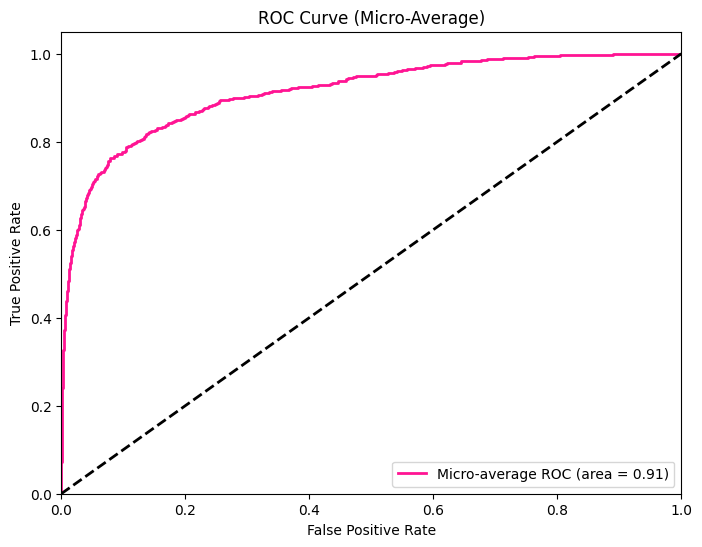
\includegraphics[width=0.65\textwidth]{roc.png}
\caption{ROC Curve}
\end{figure}

\begin{figure}[H]
\centering
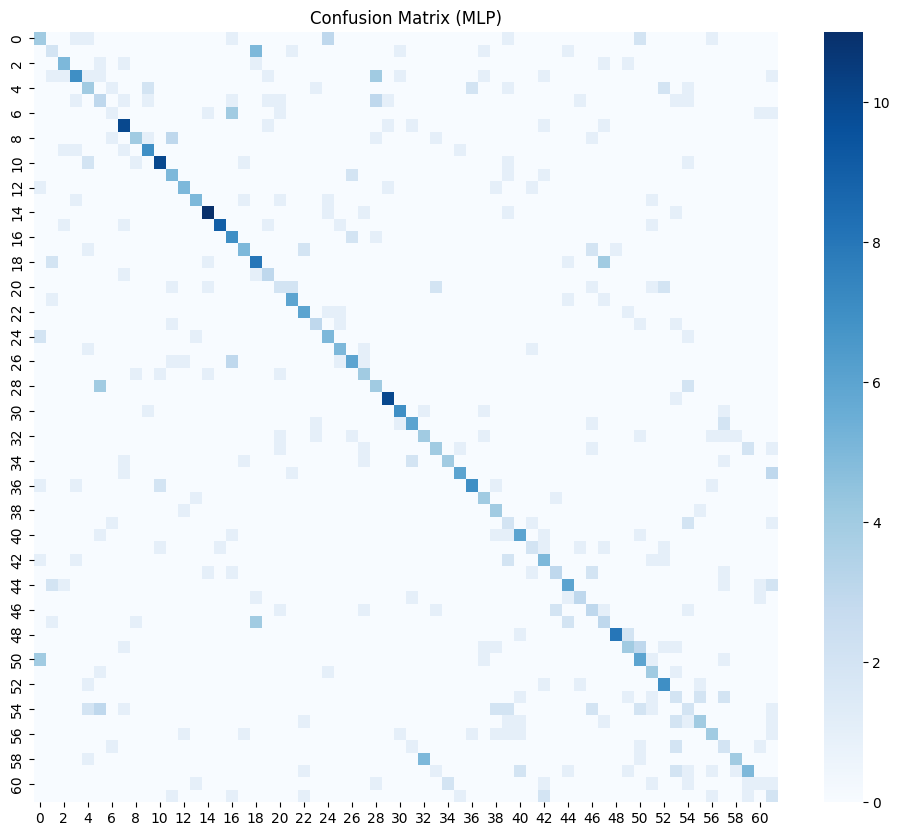
\includegraphics[width=0.75\textwidth]{confusion_matrix.png}
\caption{Confusion Matrix}
\end{figure}

\begin{figure}[H]
\centering
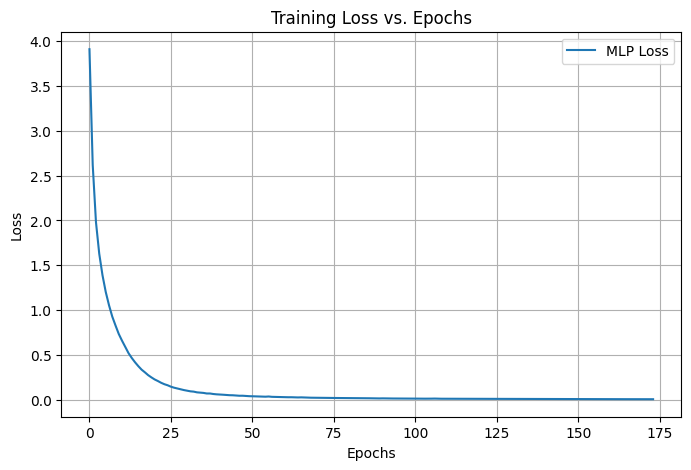
\includegraphics[width=0.75\textwidth]{training_loss.png}
\caption{Training Loss Curve}
\end{figure}
\section*{Observations}

\begin{itemize}
    \item \textbf{Why does PLA underperform compared to MLP?} \\
    PLA is a strictly linear classifier. The pixel data of handwritten characters is highly non-linear (for example, the geometric difference between an `8' and a `B' cannot be separated by a single straight line in high-dimensional space). The MLP uses hidden layers and non-linear activation functions to transform the feature space, enabling effective separation of classes.
    
    \item \textbf{Which hyperparameter had the most impact on MLP performance?} \\
    The choice of optimizer (SGD vs.\ Adam) and the learning rate had the most significant impact. Switching from SGD to Adam allowed dynamic adjustment of learning rates for each parameter, improving optimization and avoiding poor local minima.
    
    \item \textbf{How does optimizer choice affect convergence?} \\
    Standard SGD updates all weights using a fixed learning rate, which can cause slow or unstable convergence. Adam combines momentum and adaptive learning rates, leading to faster, smoother, and more stable convergence behavior.
    
    \item \textbf{Does increasing hidden layers always improve performance?} \\
    No. While deeper networks can model more complex patterns, adding too many layers can result in overfitting and the vanishing gradient problem, making training difficult without advanced techniques.
    
    \item \textbf{How can overfitting be detected and mitigated?} \\
    Overfitting is observed when training accuracy is very high but validation/test accuracy is significantly lower, often accompanied by increasing validation loss. It can be mitigated by reducing model complexity, applying dropout, using L2 regularization (weight decay), or implementing early stopping.
\end{itemize}

\section*{Conclusion}

This experiment demonstrated the transition from linear models to deep neural networks. While the PLA is conceptually important, it is not suitable for complex tasks such as handwritten character recognition. In contrast, the MLP, with proper hyperparameter tuning and modern optimization techniques, effectively handled the non-linear classification problem, achieving stable convergence and significantly improved accuracy.
\end{document}
